\begin{figure*}[t]
  \centering
  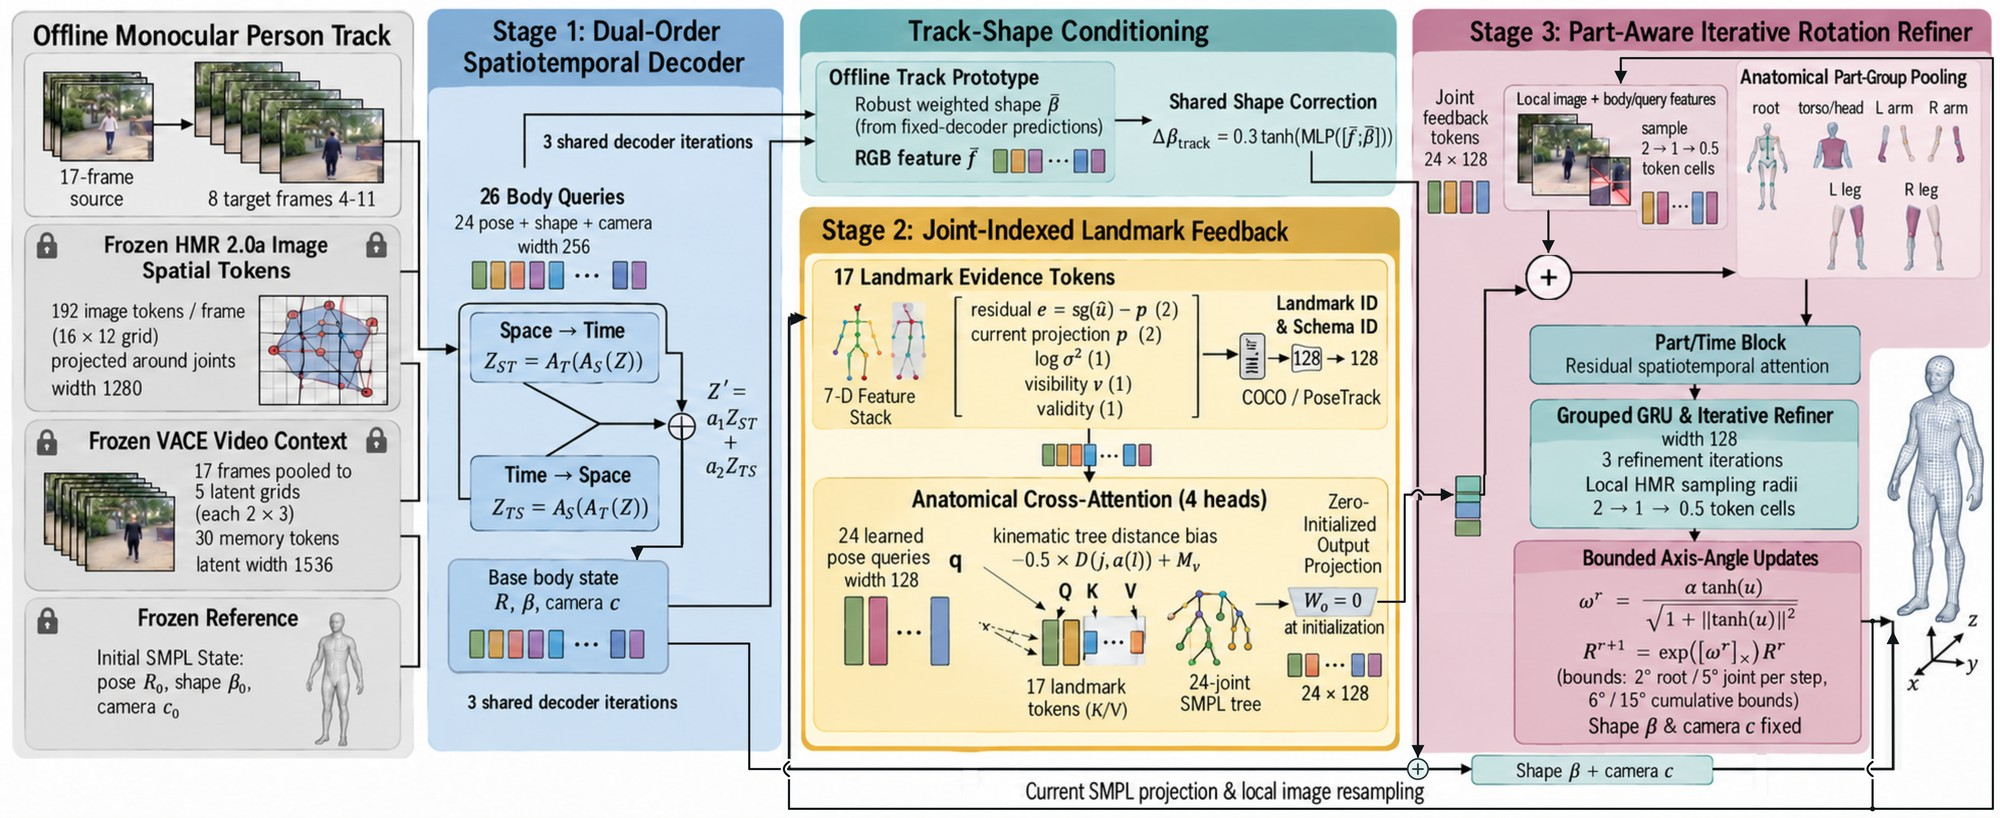
\includegraphics[width=\textwidth]{figures/overview_final.jpg}
  \caption{\textbf{\method overview.}
  A frozen dual-order spatiotemporal decoder reads HMR\,2.0a image tokens and Wan/VACE video context and predicts a residual to a frozen reference body; a track-conditioned residual shares shape over a person track.
  The final stage refines rotations for three iterations: landmark evidence is routed to 24 joint queries, added before part pooling and masked temporal exchange, and converted into bounded axis-angle updates; projections and local image samples are recomputed at every iteration.
  \TODO{Redraw stage~2 for C11: evidence tokens come from an external detector (residual $u{-}p$, projection $p$, $-2\log c$, $c$, validity) instead of the inherited head; the drawn step bounds $2^\circ/5^\circ$ are the scales $\alpha$, the tight cumulative bounds are $5.2^\circ/13.0^\circ$ (\cref{sec:refiner}).}}
  \label{fig:overview}
\end{figure*}

\section{Method}
\label{sec:method}

\subsection{Setting and inherited model}
\label{sec:setting}

Given an offline monocular person track, \method predicts for every target frame $t$ a camera-space SMPL state $x_t=(R_t,\beta_t,c_t)$ with 24 joint rotations, ten shape coefficients and a crop camera $c_t=(s_t,t_{x,t},t_{y,t})$.
All variants in this paper share one trained \emph{parent}, which we keep fixed and describe only briefly.
Each eight-frame target window reads 192 HMR\,2.0a tokens per frame~\cite{goel2023hmr2} and a 17-frame Wan/VACE context~\cite{wan2025wan,jiang2025vace} compressed to 30 memory tokens; both encoders are frozen, and the video-generation models Wan and VACE serve only as feature extractors.
Twenty-six body queries $Z$ (24 pose, shape, camera) are decoded by blocks that mix a spatial-first order $Z_{\mathrm{ST}}=A_T(A_S(Z))$ and a temporal-first order $Z_{\mathrm{TS}}=A_S(A_T(Z))$ of attention,
\begin{equation}
  Z' = a_1 Z_{\mathrm{ST}} + a_2 Z_{\mathrm{TS}},\qquad a=\softmax\big(g([Z_{\mathrm{ST}};Z_{\mathrm{TS}}])\big),
  \label{eq:dual}
\end{equation}
over three weight-shared iterations that predict a residual to a frozen reference body, using the continuous 6D rotation representation~\cite{zhou2019continuity}.
A track-conditioned residual, bounded componentwise by 0.3, maps a fixed prediction-and-image prototype of the track to a shape correction shared by all of its frames.
The final stage, a part-aware recurrent rotation refiner (\cref{sec:refiner}), is where landmark evidence enters; only its feedback module differs between variants.

\subsection{What did joint-indexed feedback route?}
\label{sec:audit}

This earlier variant, denoted C10, read 17 landmark observations $\hat u_{tl}$ from an observation head of the parent, together with a log-variance and a visibility logit, and formed the residual $\sg(\hat u_{tl})-p_{tl}(x^r)$ to the current projection $p_{tl}(x^r)$.
Every 2D loss weight was zero in all stages that produced the parent and C10, so the head never received gradient.
Its coordinate layers remain at their zero initialisation, which makes $\hat u_{tl}$ the projection of the frozen reference body; the log-variance stays at its bias of $-4$ and the visibility at $\sigma(0)=0.5$.
The routed residual is therefore $p_{tl}(x^{\text{ref}})-p_{tl}(x^r)$: the image-plane drift of the current body from the reference, with constant uncertainty features.
\TODO{confirm on the archived parent, C00 and C10 checkpoints with scripts/inspect\_checkpoint\_v43.py; report the measured verdict (all coordinate weights exactly zero, log-variance bias $-4$) here and in Supp.~S5.}
Such a signal can still help a refiner, for instance as a learned pull towards the reference, but it contains no image evidence, so an advantage of routing it cannot be attributed to evidence assignment.
Two further limitations affect the archived comparison: the mean-feedback control (C00) mapped four averaged scalars through 512 parameters, against 105,472 for the router, and both runs used a single seed with validation-only evaluation.
Relative to its parent, archived C10 changed validation MPJPE by $-0.07$\,mm with a sequence-bootstrap 95\% interval of $[-0.21, +0.03]$ (Supp.~S5).
We keep this self-referential router as variant \vA{2} and its mean control as \vA{1}, and build the method below on external evidence.

\begin{figure*}[t]
  \centering
  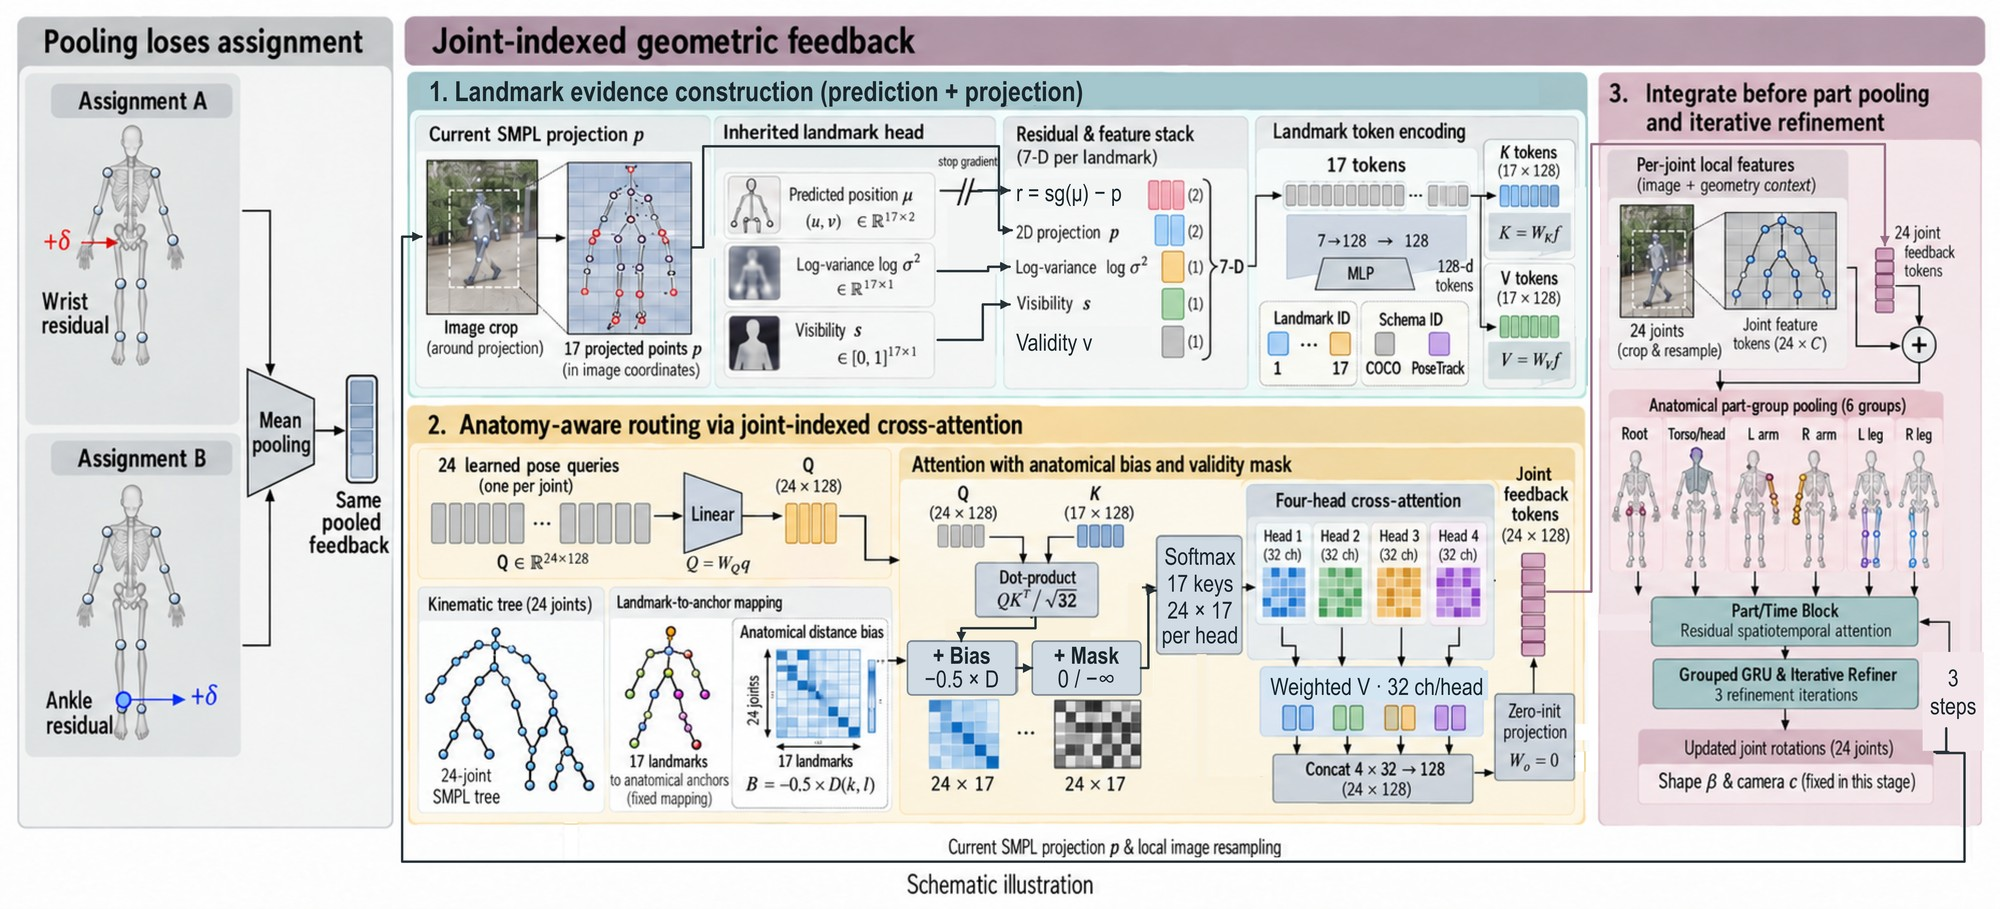
\includegraphics[width=0.88\textwidth]{figures/identity_final.jpg}
  \caption{\textbf{Identity-preserving routing} (schematic).
  Left: exchanging a wrist and an ankle residual leaves a mean-pooled feedback vector unchanged.
  Right: every landmark becomes a token with identity and schema embeddings; 24 joint queries read the 17 tokens through four-head attention with the kinematic-tree bias $-D/2$ and a validity mask, and the zero-initialised output is added to each joint before part pooling and the recurrent update.
  \TODO{Redraw panel~1 for C11: the evidence comes from an external detector (ViTPose keypoints $u$ and confidences $c$) instead of the inherited landmark head.}}
  \label{fig:identity}
\end{figure*}

\subsection{Identity-bearing evidence tokens}
\label{sec:tokens}

An external top-down detector, ViTPose~\cite{xu2022vitpose,xu2024vitposepp} (ViTPose++-H, COCO-17 expert), runs on the same $256\times256$ crop as the image backbone and returns, for each landmark $l\in\{1,\dots,17\}$, a position $u_{tl}$ in normalised crop coordinates and a confidence $c_{tl}\in[0,1]$.
Let $p_{tl}(x^r)$ be the COCO landmark regressed from the current SMPL mesh at refinement iteration $r$ and projected with the crop camera.
Each landmark becomes a seven-dimensional feature
\begin{equation}
  \phi^r_{tl} = \big[\,u_{tl}-p_{tl}(x^r);\; p_{tl}(x^r);\; -2\log c_{tl};\; c_{tl};\; v_{tl}\,\big],
  \label{eq:token}
\end{equation}
where $v_{tl}$ marks finite keypoints with positive confidence in valid frames, invalid entries are zeroed, and residual, projection and log-confidence are clipped to $[-2,2]$, $[-4,4]$ and $[-6,6]$.
The term $-2\log c$ plays the role of a log-variance and vanishes for confident detections.
A two-layer MLP maps $\phi^r_{tl}$ to width 128, and a learned landmark embedding $e_l$ plus a schema embedding are added, so that the token $z^r_{tl}$ carries its anatomical identity independently of its content.
Because $p_{tl}(x^r)$ is recomputed from the current body, the residual shrinks or changes direction as the refiner moves the joints; the evidence is a closed-loop signal rather than a fixed input.

\subsection{Anatomically biased routing}
\label{sec:routing}

Twenty-four learned joint queries $q_j$ read the evidence tokens of a person-frame with four-head attention (\cref{fig:identity}),
\begin{equation}
  A^h_{jl} = \softmax_l\!\Big(\frac{(W^h_Q q_j)^{\!\top} W^h_K z^r_{tl}}{\sqrt{d_h}} - \frac{D(j,a(l))}{2} + M_{tl}\Big),
  \label{eq:route}
\end{equation}
with $d_h=32$, where $a(l)$ is the anatomical anchor of landmark $l$ (the head joint for facial landmarks and the corresponding SMPL joint for limb landmarks), $D$ the shortest-path distance on the SMPL kinematic tree and $M_{tl}\in\{0,-\infty\}$ the validity mask.
The bias favours nearby anatomy without forbidding long-range reads, \eg a wrist query may still consult the shoulder.
The attention-weighted values of the four heads are concatenated, projected, and mapped by a final matrix $W_o$ to 24 joint feedback vectors $f^r_{tj}\in\mathbb{R}^{128}$.
We initialise $W_o=0$, so the feedback is exactly zero at the start of training while $W_o$ receives gradient immediately; together with zero-initialised residual blocks, every variant reproduces the parent's predictions before its first update.
A frame without any valid landmark receives zero feedback.
The router trains 105,472 parameters, as many as C10.
For fusion with the inherited head (\vB{6}), the 17 head tokens and the 17 external tokens, each with their own identity embeddings and anchors, form one set of 34 tokens.

\paragraph{Controls as single-factor changes.}
Every control keeps the token features of \cref{eq:token} and the zero-initialised output, and changes one factor (\cref{tab:main,tab:ablation}).
The \emph{pooled} control (\vB{1}) removes identity and routing: the per-token MLP outputs are averaged over valid landmarks, as in Deep Sets~\cite{zaheer2017deepsets}, passed through a 128--256--128 MLP and broadcast to all joints (100,096 parameters).
The \emph{ordered-vector} control (\vB{7}) keeps identity by position: the 17 encoded tokens are concatenated in slot order, mapped by a linear layer and an MLP, and broadcast to all joints, mirroring how keypoints condition WHAM-style models (329,344 parameters, $3.1\times$ the router).
The \emph{set} control (\vB{2}) keeps the joint queries but removes identity embeddings and bias, which yields Set-Transformer-style pooling by attention~\cite{lee2019settransformer} that is invariant to permuting landmarks.
\vB{3} keeps identity but removes the bias, and \vB{5} keeps identity with a bias whose landmark columns are permuted by a fixed derangement, \ie a wrong anatomy with identical bias statistics.
Note that the projected coordinates $p_{tl}$ may reveal identity implicitly even when embeddings are removed; \vB{1} and \vB{2} therefore test whether \emph{explicit} identity and routing help at this budget, not whether identity is recoverable in principle.

\subsection{Part-aware iterative rotation refinement}
\label{sec:refiner}

At iteration $r$, each joint feature combines its contextual pose query, the current body state and local HMR\,2.0a samples around its projection, whose radius shrinks from two to one to half a token cell.
The routed feedback $f^r_{tj}$ is added to this per-joint feature \emph{before} the joints are pooled into six anatomical groups (root, torso/head, two arms, two legs).
Two residual blocks then exchange information across groups within a frame and across time within a group; temporal attention is masked by source-frame identities so that duplicated or invalid frames and track gaps never act as independent evidence.
The group context is broadcast back to the joints, and a group-specific GRU, whose state persists over the three refinement iterations rather than over video frames, predicts $u^r_{tj}\in\mathbb{R}^3$, converted to a bounded axis-angle increment,
\begin{equation}
  \omega^r_{tj} = \alpha_j\,\frac{\tanh u^r_{tj}}{\sqrt{1+\lVert\tanh u^r_{tj}\rVert^2}},\qquad R^{r+1}_{tj} = \exp([\omega^r_{tj}]_\times)\,R^r_{tj},
  \label{eq:bound}
\end{equation}
with $\tanh$ applied componentwise and $\alpha_j=2^\circ$ for the root and $5^\circ$ otherwise.
Since $\lVert\tanh u\rVert<\sqrt3$ and $s/\sqrt{1+s^2}$ is increasing, each increment is smaller than $\tfrac{\sqrt3}{2}\alpha_j$, \ie $1.73^\circ$ for the root and $4.33^\circ$ for other joints, and the triangle inequality on rotations bounds the displacement after three iterations by $5.2^\circ$ and $13.0^\circ$ relative to the refiner input.
Shape and camera pass through unchanged, while projections, local samples and the routed evidence are recomputed after every update.

\paragraph{Objective.}
All variants use one objective: joint and vertex errors in metres, rotation and shape supervision, velocity and acceleration of the hip-centred prediction-minus-target joint error, a Procrustes-aligned joint auxiliary, intermediate decoder supervision and small consistency and update penalties (coefficients in Supp.~S2).
Every person-frame is owned by one window, and acceleration triplets that straddle window boundaries are retained by forwarding their owner contexts, so the motion objective and metric cover complete sequences.
No 2D reprojection loss is used; external keypoints act only as inputs.
